%----------------------------------------
% Write your notes here
%----------------------------------------

\section{Naive Bayes}
Here we saw Naive Bayes (independent assumption over all words). We predict class c given features. 

Bayes Rule:
\begin{equation}
P( c|x) = p(\bar{x}|c)\times{p(c)/p(\bar{x})}
\end{equation}
The naive part says the following:  
\begin{equation}
p(\bar{x}|c)=\prod_{j}{ p(x_{j}|c)}
\end{equation}
and then we have:
\begin{equation}
 p(c|\bar{x})=\prod_{j}{ p(x_{j}|c)}\times{p(c)/p(\bar{x})}
\end{equation}

$p(x_{j}|c)$ models a a coinflip (i.e. Bernoulli)

The word occurrences are coinflips:
\begin{equation}
p(x_{j}|c)=\theta_{jc}^{x_{j}}(1-\theta_{jc})^{1-x_{j}}
\end{equation}
$\theta_{jc}$ predicts the jth word in some class c.

 \begin{equation}
 log(p(c|x)) = \sum\limits_{j}log[\theta_{jc}^{x_{j}}(1-\theta_{jc})^{1-x_{j}}] + log [\frac{\theta_{c}}{p(\bar{x})}]
 \end{equation}
 
 \begin{equation}
= \sum\limits_{j}x_{j}log\frac{\theta_{jc}}{1-\theta_{jc}} +
 \sum\limits_{j} log(1-\theta_{jc}) + + log [\frac{\theta_{c}}{p(\bar{x})}]
 \end{equation}
 
The leftmost term is the number of words in the document; the middle term is size of the vocab. we are working with. 

We have two cases:
\begin{equation}
log\frac{p(c=1|x)}{p(c=0|\bar{x})} = \sum\limits_{j}log[\frac{\theta_{j1}(1-\theta_{j0})}{\theta_{j0}(1-\theta_{j1})}] + \sum\limits_{j}log[\frac{(1-\theta_{j1})}{(1-\theta_{j0})}] + log[\frac{\theta_{1}}{\theta_{0}}]
\end{equation}

Let's look at the difference of the log prob. of both of our cases:
Lets define:
\begin{equation}
w_{j} = log[\frac{\theta_{j1}(1-\theta_{j0})}{\theta_{j0}(1-\theta_{j1})}]
\end{equation}

So we end up with:
\begin{equation}
log\frac{p(c=1|\bar{x})}{p(c=1|\bar{x})} = \bar{x}\cdot\bar{w_{j}} +\bar{w_{0}}
\end{equation}

Calculate $\theta_{j}$
To do this we will take the derivative of the log-likelihood of the probability of seeing n heads:

\begin{equation}
0 = \frac{n}{\theta} + \frac{N - n}{1 - \theta}
\end{equation}

\begin{equation}
\theta_{j1}=\frac{n_{j1}}{n_{1}}=\frac{\textnormal{num of spam docs w/ word j}}{\textnormal{num of spam docs}}
\end{equation}

\begin{equation}
\theta_{1}=\frac{n_{1}}{N}=\frac{\textnormal{num of spam docs}}{\textnormal{num of total docs}}
\end{equation}

\section{Logistic Regression}
We shall begin here with the predictor we got above: 
\begin{equation}
\log{\frac{P}{1-p}} = w\cdot x
\end{equation}

\begin{equation}
p = \frac{1}{1+e^{-w\cdot x}}
\end{equation}
\begin{figure}[ht]
  \begin{center}
    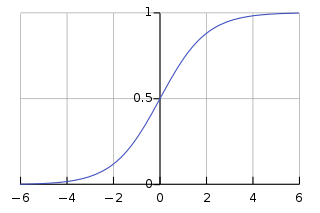
\includegraphics[width=0.5\textwidth]{figures/pic1.png}
    \caption{
      A graph of th Sigmoid Function (from Wikipedia). 
      }
    \label{fig:example_figure}
  \end{center}
\end{figure}
We have a set of documents $x_i$ and a set of labels $y_i$, we know find the model.
\begin{equation}
\textnormal{LL} = P(D|w) = \prod_{i} {p_{i}^{y_{i}} (1-p_{i}) ^ {1-y_{i}}}
\end{equation}

Using the above equations and taking the log likelihood we get:
\begin{equation}
L= -\sum_i[y_iw\cdot x -(\log{1 + e^{w \cdot x}})]
\end{equation}

We set the derivative to zero to find the max likelihood and end up with:
\begin{equation}
0 = -\sum_i[y_i\cdot x -(\frac{1}{1 + e^{w \cdot x}})]x_{ik}
\end{equation}

We use Gradient Descent, since no solution exists:
\begin{equation}
w = w - n\frac{\partial L}{\partial w}
\end{equation}

It is also:

\begin{equation}
w_k  = w_k + n\sum_i[(y_i - p_i)x_{ik}]
\end{equation}

We can regularize the model as well as follows:

\begin{equation}
L = \sum_i [y_i log _i+(1-y_i)log(1-p_i)]+0.5\lambda{}||w||^{2}
\end{equation}

\begin{equation}
\frac{\partial L}{\partial w_k}=\sum_i[(y_i-p_i)x_{ik}]+\lambda{}w_k 
\end{equation}

We thus end of with: 
\begin{equation}
w_k = (1 - n\lambda{})w_k + n \sum_i[(y_i-p_i)x_{ik}]
\end{equation}


\section{Evaluation}

When evaluating various classifiers we can consider a number of things:
\begin{itemize}
\item Accuracy: The fraction of times we predict the correct label.
\item Calibration: This is how often an event with predicted probability p occurs.
\item Confusion Matrix:
\begin{equation}
p = \frac{1}{1+e^{-w\cdot x}}
\end{equation}
\begin{figure}[ht]
  \begin{center}
    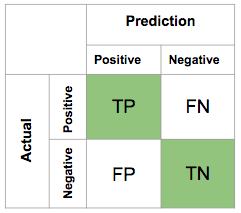
\includegraphics[width=0.5\textwidth]{figures/pic2.png}
    \caption{
      A Confusion Matrix (from WS02). 
      }
    \label{fig:example_figure2}
  \end{center}
\end{figure}

\item Receiver Operating Characteristic (ROC) curve: ROC curve plots the true positive rate and the false positive rate
\begin{figure}[ht]
  \begin{center}
    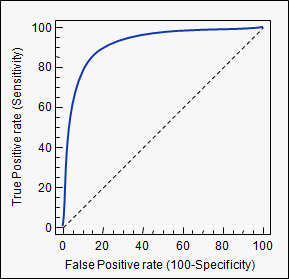
\includegraphics[width=0.5\textwidth]{figures/pic3.png}
    \caption{
      ROC Curve (from Wikipedia). 
      }
    \label{fig:example_figure3}
  \end{center}
\end{figure}
\end{itemize}



